\chapter{\ifenglish Introduction\else บทนำ\fi}

\section{\ifenglish Project rationale\else ที่มาของโครงงาน\fi}
\par จากระบบการขายสินค้าในร้านค้าปลีกส่วนใหญ่ของประเทศไทย ไม่ว่าจะเป็นห้างสรรพสินค้า ซุปเปอร์มาเก็ต หรือ
ร้านค้าปลีกรายย่อยต่าง ๆ พบว่าวิธีการที่ใช้ในการชำระสินค้า คือ การชำระสินค้าที่เคาน์เตอร์ชำระเงินโดยมีพนักงานบริการ 
ซึ่งข้อเสียแรกของวิธีการชำระสินค้าดังกล่าว คือ การรอชำระสินค้าที่แคชเชียร์นั้นเสียเวลา และไม่สะดวกรวดเร็ว 
ยิ่งหากต้องมีการต่อแถวรอชำระเงิน ก็จะทำให้ผู้ใช้บริการเสียเวลามากขึ้น และเสียความพึงพอใจในการใช้บริการ 
รวมถึงต้องมีการจัดพื้นที่สำหรับการต่อแถวอีกด้วย ด้วยเหตุนี้ จึงควรพัฒนาเทคโนโลยีที่มาช่วยการแก้ปัญหาอย่างตรงจุด 
โดยให้ลูกค้าสามารถชำระสินค้าได้ด้วยตนเอง self-service\enskip
 หลังการเลือกซื้อสินค้าได้อย่างสะดวกสบายผ่านอุปกรณ์โทรศัพท์มือถือ 
\par นอกจากนี้สำหรับร้านค้าปลีกรายย่อยที่มีรูปแบบการขายเป็นแบบบริการตนเอง หรือแม้กระทั่งร้านค้าปลีกที่มีพนักงานชำระเงิน
แต่ไม่มีระบบช่วยจัดการยอดขาย ก็สามารถพบปัญหาในการจัดการยอดขาย และคลังสินค้าได้ เนื่องจากพนักงาน
 หรือเจ้าของร้านต้องติดตามการขายสินค้าด้วยตนเองทั้งหมด โดยจะต้องคอยนับจํานวนสินค้าที่เหลืออยู่ภายในร้านเพื่อตรวจสอบว่าได้ขายอะไรไปแล้ว
  ทำให้เกิดความยากลำบาก และผิดพลาดได้ง่าย 
\par ผู้จัดทําจึงพัฒนาระบบ CapSnap self-service เพื่อลดปัญหาที่เกิดจากการรอชำระเงินที่แคชเชียร์ 
โดยพัฒนาแอพลิเคชันสำหรับผู้ใช้งานทั่วไปที่สามารถเชื่อมต่อกับร้านค้าที่เข้าร่วมเพื่อใช้บริการการซื้อสินค้าแบบ self-service 
ที่ร้านค้านั้น ๆ โดยลูกค้าสามารถเข้าใช้งานแอพลิเคชันในโทรศัพท์มือถือแล้วทำการเลือกซื้อสินค้าผ่านฟังก์ชันการสตรีมมิ่งภาพสินค้าเพื่อ
ทราบถึงรายละเอียดของสินค้า และเพิ่มสินค้าเข้าตะกร้า โดยระบบจะใช้หลักการทาง Computational Intelligence ในการแยกแยะสินค้า
จากการสตรีมมิ่ง ลูกค้าสามารถชำระเงินได้ด้วยตนเองพร้อมนำสินค้าที่ซื้อออกจากร้านค้าได้เลย ซึ่งระบบจะเก็บบันทึกประวัติการขายสินค้าลง
ในฐานข้อมูลเพื่อแสดงให้กับฝั่ง Website Dashboard ของร้านค้าซึ่งสามารถบริการจัดการคลังสินข้า และข้อมูลการขายได้ในที่เดียว 
เพิ่มประสบการณ์การใช้บริการที่ดีให้ลูกค้า และเพิ่มประสิทธิภาพในการบริหารจัดการสินค้าในร้านค้าสำหรับร้านค้าที่ต้องการให้บริการแบบ
 self-service ลดการว่าจ้างพนักงาน และต้องการเครื่องมือในการบริหารร้านค้า 
 


\section{\ifenglish Objectives\else วัตถุประสงค์ของโครงงาน\fi}
\begin{enumerate}
    \item เพื่อพัฒนาระบบ แยกแยะชนิดสินค้าโดยใช้ Computational Intelligence ได้
    \item เพื่อสร้างเว็บไซต์และแอปโทรศัพท์เพื่อให้ผู้ใช้งานสามารถใช้งานระบบได้
\end{enumerate}

\section{\ifenglish Project scope\else ขอบเขตของโครงงาน\fi}
ข้อมูลที่ใช้ในการฝึกระบบ Computational Intelligence ในการแยกแยะชนิดสินค้า
เป็นชุดข้อมูลที่เก็บจากร้านค้าห้อง 422 ตึก 30 ปี คณะวิศวกรรมศาสตร์ สาขาวิชาวิศวกรรมคอมพิวเตอร์ มหาวิทยาลัยเชียงใหม่  
% \subsection{\ifenglish Hardware scope\else ขอบเขตด้านฮาร์ดแวร์\fi}

% \subsection{\ifenglish Software scope\else ขอบเขตด้านซอฟต์แวร์\fi}

\section{\ifenglish Expected outcomes\else ประโยชน์ที่ได้รับ\fi}
\begin{enumerate}
    \item แอพลิเคชันในโทรศัพท์มือถือที่ลูกค้าสามารถแยกแยะชนิดสินค้าเพื่อให้ลูกค้าสามารถจ่ายเงินให้กับสินค้านั้นๆได้ด้วยตัวเอง โดยไม่ต้องคอยเลือกชนิดของสินค้านั้นๆ
    \item เว็บไซต์ที่แสดงจำนวนการขายของสิ้นค้าแต่ละชนิดเพื่อให้ร้านค้าสามารถจัดการสินค้าได้
\end{enumerate}
\section{\ifenglish Technology and tools\else เทคโนโลยีและเครื่องมือที่ใช้\fi}
\begin{enumerate}
    \item Python และ Aiortc : สำหรับพัฒนาในส่วนของ Backend การรับข้อมูลสตรีมมิ่งจากแอพลิเคชัน การฝึกสอนโมเดล และการ classify Product
    โดยไม่ต้องคอยเลือกชนิดของสินค้านั้นๆ
    \item Flask และ Next.js: สําหรับการพัฒนา Frontend ในส่วนเว็บไซต์ของร้านค้า (Website Dashboard)
    \item Flutter แลพ Webrtc: สำหรับพัฒนา Frontend  ในส่วน Application ในโทรศัพท์มือถือของลูกค้า และใช้ Webrtc ในการสตีมมิ่งภาพจากกล้องโทรศัพท์มือถือไปยังส่วน Backend เพื่อทำการประมวลผล
    \item Supabase: สําหรับเก็บฐานข้อมูลทั้งหมดที่แสดงผล

\end{enumerate}
% \subsection{\ifenglish Hardware technology\else เทคโนโลยีด้านฮาร์ดแวร์\fi}

% \subsection{\ifenglish Software technology\else เทคโนโลยีด้านซอฟต์แวร์\fi}


\section{\ifenglish Project plan\else แผนการดำเนินงาน\fi}
% \begin{table}[h]
%     % 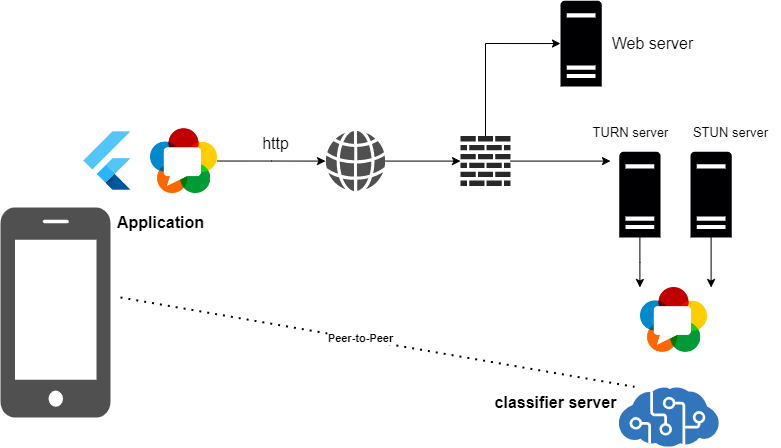
\includegraphics{pic/webrtc.png}
%     \begin{plan}{1}{2023}{3}{2024}
%         \planitem{1}{2023}{2}{2023}{Planning}
%         \planitem{3}{2023}{3}{2023}{Document}
%         \planitem{2}{2023}{3}{2023}{Back-end development}
%         \planitem{5}{2023}{6}{2023}{App development}
%         \planitem{11}{2023}{12}{2023}{Dashboard development}
%         \planitem{1}{2024}{3}{2024}{Testing}
%     \end{plan}
    
%     \caption[Planning]{Planning}
%     \label{table:Planning}
%     \end{table}
    \begin{table}[h]
        \begin{center}
        % 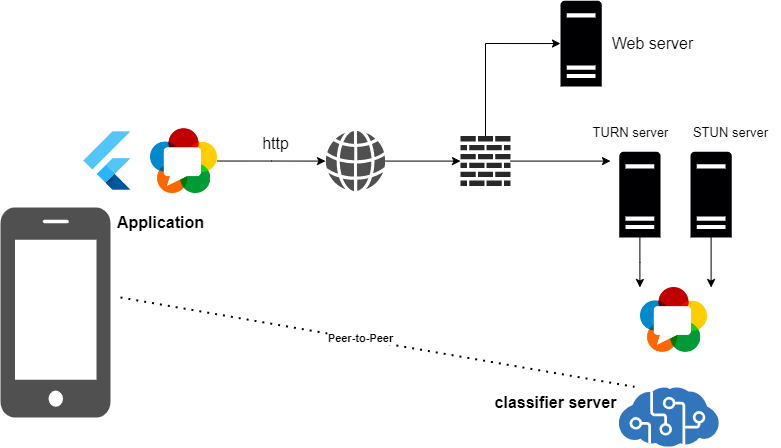
\includegraphics{pic/webrtc.png}
        \vspace{0.5cm}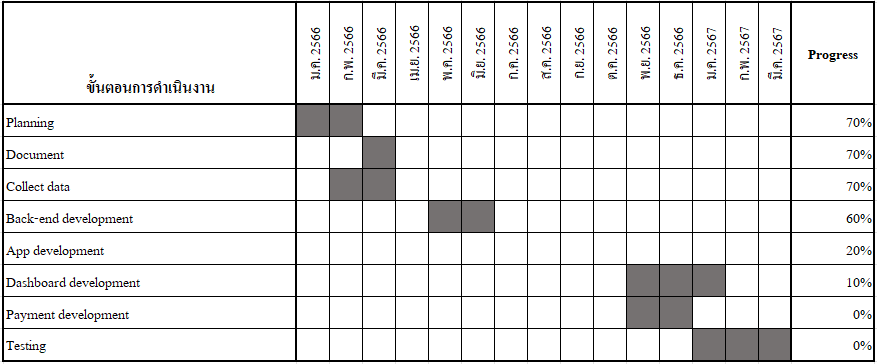
\includegraphics[scale=0.64]{pic/plane.png}
        \end{center}
        
        \caption[Planning]{Planning}
        \label{table:Planning}
        \end{table}

\newpage
\section{\ifenglish Roles and responsibilities\else บทบาทและความรับผิดชอบ\fi}
นายพงศกร รัตนพันธ์ รหัส 630610749 รับผิดชอบในส่วนของ Backend ดังนี้

\begin{enumerate}
    \item การรับข้อมูลสตรีมมิ่งจากระหว่าง Mobile Application และ  Classifier ผ่าน WebRTC
    \item การฝึกสอนโมเดลเพื่อทำ Product classification
    \item การจัดเก็บฐานข้อมูลข้อมูลรูปภาพของสินค้าเพื่อทำการฝึกสอนโมเดล
\end{enumerate}


นางสาวศุภริฎา  ศิลปสิทธิ์ รหัส 630610765 รับผิดชอบการพัฒนาส่วน Frontend และ ฐานข้อมูลบน Supabase ดังนี้
\begin{enumerate}
    \item ทั้งหน้าเว็บไซต์ของร้าน (website dashboard) 
    \item Mobile Application
    \item จัดการการเก็บฐานข้อมูลทั้งหมดที่ใช้ในการแสดงผล
\end{enumerate}
\section{\ifenglish%
Impacts of this project on society, health, safety, legal, and cultural issues
\else%
ผลกระทบด้านสังคม สุขภาพ ความปลอดภัย กฎหมาย และวัฒนธรรม
\fi}

\par โครงการนี้ลดความซับซ้อนและเวลาที่ลูกค้าจะต้องรอต่อแถวเพื่อจ่ายเงินของสินค้า
% รวมถึงทำให้พนักงานของร้านค้า ไม่ต้องคอยนับจำนวนสินค้าในร้านค้า  ในร้านค้าที่เป็นระบบ Self-Service  
% อีกทั้งยังเป็นอักทางเลือกหนึ่งในการที่ร้านค้าจะมาใช้ระบบ Self-Service ที่มีการจัดการที่ดี และ ส่งเสริมวัฒนธรรมในการบริการตนเองของลูกค้า
และ ช่วยให้สังคมสามารถเข้าถึงเทคโนโลยีที่ก้าวหน้าไปจากเดิมในการใช้กิจวัตรประจำวันอย่างการซื้อสินค้า
โดยเปลี่ยนมาใช้การบริการตนเองผ่านแอพลิเคชันที่อำนวยความสะดวกผ่านอุปกรณ์มือถือที่ใช้งานกันอย่างแพร่หลาย 
ทำให้สังคมคมก้าวสู่ความทันสมัย และความสะดวกสบายมากขึ้น ตอบโจทย์ความต้องการ และรูปแบบการใช้ชีวิตของผู้คนในยุคสมัยใหม่ 
ช่วยหลีกเลี่ยงปัญหาทางสุขภาพกาย ที่อาจเกิดจากการยืนรอชำระสินค้า หรือการใช้สายตาในการหาข้อมูลสินค้า 
และพัฒนาสุขภาพจิตจากประสบการณ์การซื้อสินค้าที่ดีขึ้น 
\par อีกทั้งยังเป็นอักทางเลือกหนึ่งในการที่ร้านค้าจะมาใช้ระบบ self-service ที่มีการจัดการที่ดี
เจ้าของกิจการร้านค้าปลีกสามารถจัดการบริหารร้านค้าได้สะดวก 
และมีประสิทธิภาพมากขึ้น ทำให้เกิดความคุ้นเคยกับวัฒนธรรมการซื้อของแบบบริการตนเองในสังคมประเทศไทยมากขึ้น 
รวมถึงเป็นต้นแบบในการพัฒนาโครงการในลักษณะเดียวกันเพื่อความก้าวหน้าทางเทคโนโลยีในประเทศต่อไป